%===============================================================================
% Zweck:    KTR-Seminar-Vorlage
% Erstellt: 16.10.2007
% Updated:  15.04.2013
% Autor:    U.K. / M.G.
%===============================================================================

%===============================================================================
% Zum Kompilieren pdflatex und bibtex ausführen.
%	Konfiguration: in texmaker unter Benutzer -> Benutzerbefehle einen neuen Befehl anlegen: pdflatex -synctex=1 -interaction=nonstopmode %.tex | bibtex % | makeindex %.nlo -s nomencl.ist -o %.nls | pdflatex -synctex=1 -interaction=nonstopmode %.tex | pdflatex -synctex=1 -interaction=nonstopmode %.tex
%	Entsprechende Informationen in den config/metainfo verändern
% Zur Auswahl der Sprache im folgenden Befehl
% ngerman für deutsch eintragen, english für Englisch.
%===============================================================================

% Options ngerman, english
\newcommand{\lang}{english}

\documentclass[pdftex, journal, onecolumn, a4paper, 12pt, \lang]{IEEEtran}

%===============================================================================
% zentrale Layout-Angaben und Befehle
%===============================================================================
% What You should change:
% Here goes your name
\author{Likitha Purushotham \\ Mahalakshmi Suravarapu \\ Pio Chibuzor Okongwu}
% and the title of your project
\title{Video Transport from Single-Board Computers like the Rasperry Pi in the Internet of Things for Web Real-Time Commuincations}
% the date of the submission
\date{October 28, 2020}

\newlanguagecommand{\semester}
\addtolanguagecommand{\semester}{english}{Summer Term 2020}
\addtolanguagecommand{\semester}{ngerman}{Sommersemester 2020}

\newcommand{\supervisor}{Prof. Dr. Udo Krieger \& Marcel Großmann}

\gitfalse

%===============================================================================
% Zweck: KTR-Seminar-Vorlage in Anlehung an G. Wirtz, Lehrstuhl Praktische Informatik
%===============================================================================
%===============================================================================
% zentrale Layout-Angaben und Befehle
%===============================================================================
%
% \usepackage{german}
\usepackage{ifthen}
% Language Selection for Babel
\ifthenelse{\equal{\lang}{ngerman}}{\usepackage[german, \lang]{babel}}{\usepackage[\lang]{babel}}

\usepackage[utf8]{inputenc}
\usepackage{fancyhdr}
\usepackage[T1]{fontenc}
\usepackage{ae}
\usepackage{color}
\usepackage{amsmath}
\usepackage{amsfonts}
%

\usepackage{caption}

%%   Fuer anspruchsvolle Tabellen   %%
\usepackage{longtable, colortbl}
\usepackage{multicol, multirow}

\usepackage[pdftitle={\@title},pdfauthor={\@author},pdftex,bookmarksopen,bookmarksnumbered,pdfborder=0]{hyperref}
\usepackage[pdftex]{graphicx}
\usepackage{float}
\usepackage{tikz}
\usepackage{pgfplots}
\usetikzlibrary{arrows,shapes,fit,positioning,snakes,backgrounds,shadows}

\pdfcompresslevel=9

% Code-Hervorhebung
% Quellcode
\usepackage{verbatim}            % Quellcode einbinden (\verbatiminput) standardpaket
\usepackage{moreverb} 
% PseudoCode
\usepackage{algorithm}
\usepackage{algpseudocode}
%\usepackage{algorithmicx}
\floatname{algorithm}{Algorithmus}
\algrenewcommand{\algorithmiccomment}[1]{\hskip1em\textcolor{gray!60}{$\rhd$ #1}}
\ifthenelse{\equal{\lang}{ngerman}}{%
\renewcommand{\listalgorithmname}{Algorithmen}
\def\algorithmautorefname{Algorithmus}
}{%
\renewcommand{\listalgorithmname}{List of Algorithms}
\def\algorithmautorefname{Algorithm}
}


%%   intoc zur Aufnhame des Abkuerzungs- und Symbolverzeichnisses ins Inhaltsverzeichnis  
\usepackage[intoc]{nomencl}
\setlength{\nomlabelwidth}{.20\hsize}
%\renewcommand{\nomlabel}[1]{#1 \dotfill}
\setlength{\nomitemsep}{-\parsep}
\makenomenclature
\ifthenelse{\equal{\lang}{ngerman}}{%
\renewcommand{\nomname}{Abk\"urzungsverzeichnis}
%\newcommand{\nomaltname}{Symbolverzeichnis}
}{%
\renewcommand{\nomname}{List of Abbreviations}
%\newcommand{\nomaltname}{List of Symbols}
}%
%\newcommand{\nomaltpreamble}{}
%\newcommand{\nomaltpostamble}{}
%\newcommand{\usetwonomenclatures}{\nomenclature[\switchnomitem]{}{}}
%\newcommand{\switchnomitem}{R}
%\renewcommand{\nomgroup}[1]{%
%\ifthenelse{\equal{#1}{\switchnomitem}}{\switchnomalt}{}}
%\newcommand{\switchnomalt}{%
%\end{thenomenclature}
%\newpage
%\renewcommand{\nomname}{\nomaltname}
%\renewcommand{\nompreamble}{\nomaltpreamble}
%\renewcommand{\nompostamble}{\nomaltpostamble}
%\begin{thenomenclature}
%}


%%   Hervorhebung der Abkuerzungsbuchstaben   %%
\usepackage[normalem]{ulem}
\newcommand{\m}[1]{\uline{#1}}

%\usepackage[dvips]{rotating}
%
% ausf\"{u}hrlichere Fehlermeldungen
\errorcontextlines=999
%
% Page-Layout: A4 aus Header
% Alternative
\setlength\headheight{14pt}
\setlength\topmargin{-15,4mm}
\setlength\oddsidemargin{-0,4mm}
\setlength\evensidemargin{-0,4mm}
\setlength\textwidth{160mm}
\setlength\textheight{252mm}
%
%% Absatzeinstellungen
\setlength\parindent{0mm}
\setlength\parskip{2ex}


\makeatletter
\renewcommand{\maketitle} {
  \begin{titlepage}
  \centering
    \begin{minipage}[t]{16cm}
      \hfill
      \begin{minipage}{12cm}
      \ifthenelse{\equal{\lang}{ngerman}}{%
        \centering
        Otto-Friedrich-Universit\"at Bamberg
        \\[12pt]%
        {\Large Professur f\"ur Informatik\\[.5em]%
        \large insbesondere Kommunikationsdienste,\\[.5em]%
        Telekommunikationsdienste und Rechnernetze}%
        }{%
        \centering
        Otto-Friedrich-University of Bamberg
        \\[12pt]
        {\Large Professorship for Computer Science,\\[.5em]%
        \large Communication Services, Telecommunication\\[.5em]%
        Systems and Computer Networks}%
        }
      \end{minipage}
      \hfill
      \begin{minipage}{3cm}
        
\includegraphics[height=28mm]{config/images/logo} %height=26mm
      \end{minipage}
    \end{minipage}\\[70pt]%[50pt]
   % 
    {\Large\bf \ifthenelse{\equal{\lang}{ngerman}}{Ausarbeitung des KTR-Seminars}{Seminar on}}
    \\[36pt]
   % oder: {\LARGE Ausarbeitung des KTR-Seminars}\\[12pt]
    {\LARGE \@title}\\[80pt]
    {\Large\bf \ifthenelse{\equal{\lang}{ngerman}}{Thema:}{Topic:}}\\[36pt]
    {\LARGE\bf \subtitle}\\
    \vfill
    \begin{minipage}{\textwidth}
      \center
      \ifthenelse{\equal{\lang}{ngerman}}{Vorgelegt von:}{Submitted by:}\\
      {\Large \@author \\[18pt]}
      \ifthenelse{\equal{\lang}{ngerman}}{Betreuer:}{Supervisor:} \supervisor \\[12pt]
      Bamberg, \@date\\
      \semester
    \end{minipage}
  \end{titlepage}
}
\makeatother
%
\usepackage[intoc]{nomencl}
\ifthenelse{\equal{\lang}{ngerman}}{%
\renewcommand{\nomname}{Abkürzungsverzeichnis}}%
{\renewcommand{\nomname}{List of Abbreviations}}
\renewcommand{\nomlabel}[1]{#1 \dotfill}
\makenomenclature

% Einbindung eines Bildes mit angegebener Breite
% #1 = label f\"{u}r \ref-Verweise
% #2 = Name des Bildes ohne Endung relativ zu Bilder-Verzeichnis
% #3 = Beschriftung
% #4 = Breite des Bildes im Dokument in cm
\newcommand{\bildw}[4]{%
  \begin{figure}[htb]%
    \centering
    \includegraphics[width=#4cm]{Bilder/#2}%
    \vskip -0.3cm%
    \caption{#3}%
    \vskip -0,2cm%
    \label{#1}%
  \end{figure}%
}
%
% Einbindung eines Bildes mit Seitenbreite
% #1 = label f\"{u}r \ref-Verweise
% #2 = Name des Bildes ohne Endung relativ zu Bilder-Verzeichnis
% #3 = Beschriftung
\newcommand{\bild}[3]{%
  \begin{figure}[htb]%
    \centering%
    \includegraphics[width=\textwidth]{Bilder/#2}%
    \vskip -0.3cm%
    \caption{#3}%
    \vskip -0,2cm%
    \label{#1}%
  \end{figure}%
}
%
\numberwithin{equation}{section}
%
%===============================================================================
% zentrale Layout-Angaben und Befehle
%===============================================================================
%
%#1 Breite
%#2 Datei (liegt im image Verzeichnis)
%#3 Beschriftung
%#4 Label fuer Referenzierung
\newcommand{\image}[4]{%
\begin{figure}[H]%
\centering%
\includegraphics[width=#1]{image/#2}%
\caption{#3}%
\label{#4}%
\end{figure}%
}

%#1 Datei (liegt im graphic Verzeichnis)
%#2 Beschriftung
%#3 Label fuer Referenzierung
%#4 Skalierungsfaktor
\newcommand{\scaletikzimage}[4]{%
\begin{figure}[H]%
\centering%
\scalebox{#4}{%
\input{graphic/#1.tikz}}%
\caption{#2}%
\label{#3}%
\end{figure}
}

%#1 algorithm name
%#2 algorithm label
%#3 file name in code-folder
\newcommand{\pseudo}[3]{%
\small%
\begin{algorithm}[H]%
\caption{#1}%
\label{#2}%
\input{code/#3.tex}%
\end{algorithm}%
\normalsize%
}


%===============================================================================
% LATEX-Dokument
%===============================================================================

\hyphenation{op-tical net-works semi-conduc-tor}
\begin{document}

\maketitle

\pagenumbering{Roman}
\setcounter{page}{2}
%
\hypersetup{hidelinks}
\tableofcontents
% Einstellungen f\"{u}r Literaturverzeichnis
\newpage
\addcontentsline{toc}{section}{\listfigurename}
\listoffigures
\newpage
%\addcontentsline{toc}{section}{\listtablename}
%\listoftables
\newpage
\printnomenclature
%===============================================================================
% LATEX-Dokument: Kapitel laden
%===============================================================================
%
\newpage
\pagenumbering{arabic}
\setcounter{page}{1}


%
% hier einzelne Kapitel mit \input{Kapitel-File} einf\"{u}gen
%
%\section{Einleitung}\label{sec:ein}
Einleitung nach \autoref{sec:ein}

\section{Hauptteil}\label{sec:haupt}
\subsection{Bilder und Grafiken}\label{subsec:grafiken}
\subsubsection{Bilder}\label{subsubsec:bilder}
Bilder befinden sich im Image-Orgner und lassen sich mit \textbackslash image\{Breite\}\{Datei im Image-Verzeichnis\}\{Beschriftung\}\{Label\} einbinden. \image{3cm}{logo.png}{Uni-Logo}{img:uni} Die Referenzierung erfolg mittels \textbackslash autoref\{Label\}, also z.B. \autoref{img:uni}.
\subsubsection{Grafiken mit TikZ}
Grafiken im TikZ-Framework\footnote{\url{http://www.tn-home.de/TUGDD/Stuff/TikZ_final.pdf}} lassen sich mit dem Befehl \textbackslash scaletikzimage\{Datei im Image Verzeichnis\}\{Beschriftung\}\{Label\}\{Skalierungsfaktor\} einbinden. \scaletikzimage{tikz}{TikZ-Grafik}{img:tikz}{0.9}
\subsection{Tabellen}
Tabellen lassen sich mit dem Environment\\
\textbackslash begin\{longtable\}[H h t b c]\{Spaltendefinitionen\} ...\\
\qquad\qquad \textbackslash caption\{Tabellenunterschrift\}\\
\qquad\qquad \textbackslash label\{Label\}\\
\textbackslash end\{longtable\}\\
 definieren\footnote{\url{ftp://ftp.dante.de/pub/tex/macros/latex/required/tools/longtable.pdf}}\\
\begin{longtable}[H]{|p{0.2\textwidth}|p{0.2\textwidth}|p{0.2\textwidth}|}
\hline
A&B&C\\
\hline
\caption{Tabelle 1}
\label{tab:tab1}
\end{longtable}
\subsection{Code-Ausschnitte}
Pseudo-Code Ausschnitte lassen sich mit \textbackslash pseudo\{Name des Algorithmus\}\{Label\}\{Datei im Code-Verzeichnis\} einbinden.
\pseudo{Mittelwert}{lst:mean}{code}
\section{Zitate}
Mit \textbackslash nocite*\{\} lassen sich alle Einträge in der Bibliography ausgeben. Mit \textbackslash cite[S. xx]\{Key\} lassen sich Zitate einfügen. Z.B. \cite[S. 234]{Kurose12} \nocite*{}
\subsection{Abkürzungen}

Abkürzungen können mit \textbackslash nomenclature\{Abk\}\{\textbackslash m\{Abk\}ürzung\} \nomenclature{Abk}{\m{Abk}ürzung} angegeben werden. Diese werden alphabetisch sortiert in ein Abkürzungsverzeichnis aufgenommen.


\section*{List of Abbreviations}
\begin{table}[ht]
\begin{tabular}{lll}
eMR & Electronic medical record \\
eHR & Electronic health record \\
DTLS & Datagram Transport Layer security \\
IT & Information Technology \\
ID & Identification \\
IaaS & Infrastructure as a Service \\
IoT & Internet of Things \\
IoHT & Internet of Healthcare Things \\
IPSec & Internet Protocol Security \\
LS & Loss-sentitive \\
OS & Operating System \\
OTrP & OpenTrust Protocol \\
PaaS & Platform as a Service \\
QoS & Quality-of-Service \\
SDN & Software-Defined Networking \\
SDNC & Software-Defined Networking controller \\
SaaS & Software as a Service \\
SSL & Secure socket layer \\
TCP & Transmission Control Protocol \\
TLS & Transport Layer Security \\
WebRTC & Web Real time communication \\
\end{tabular}
\end{table}
\newpage
\section{Introduction}\label{sec:one}
\subsection{Motivation}
The rapid growth in technology and information sector in recent years has resulted in a wide range of connectivity for various electronic and heterogeneous devices that can communicate effortlessly with each other over the internet.This is what is called as 'Internet of Things'\cite{3}.\\ \\
Due to this growth in technology,we can experience a exponential growth in the usage of devices in upcoming years that can rule over the internet.\\ \\
This technological improvement has made a gateway for various different industrial sectors including Healthcare inculcate IoT with varied applications leading to new possibilities.\\ \\
According to the recent research in healthcare industries,the life expectancy is said to increase by 31\% and the aged population is said to increase by 16\% which can result in highly vulnerable population that are prone to chronic and other diseases resulting in a large percentage of deaths and global burden inturn leading to the shortage of healthcare workforce in upcoming years.\\ \\
With this aim,several healthcare frameworks have been developed based on Internet of Healthcare Technology that can provide improved and reliable services with reduced cost,highly energy efficient and scalable solutions to meet the shortage of healthcare workforce and help in prevention of diseases,treatement and cure.\\ \\
Nonetheless,the various healthcare devices generate a huge amount of heterogeneous data that require special consideration in terms of different data specific processing power,quick response time and huge storage of data which can be a challenging task.\\ \\
In order overcome this challenge ,Taylor paper\cite{3}proposes a 5-Layered IoHT framework that consist of Perception,Mist,Fog,Cloud and Application which is capable of handling different routing paths for different data types that consists of realtime and offline/batch mode data providing optimal resource utilization,balanced network load and allocate resources as required by making use of Software defined networks(SDN).\\ \\
The results from the paper show that the proposed IoHT framework provide better QoS in terms of low power consumption,reduced latency and low packet drop rate leading to an efficient development for the existing \& next generation e-Healthcare systems.\\ \\

\section{Foundations for Our System}

%subsection1---------
\subsection{Hardware Technologies}

\subsubsection{Raspberry Pi}
The RPi\footnote{\url{https://en.wikipedia.org/wiki/Raspberry_Pi}} is a series of small SBCs which operates in an open-source ecosystem that features a Broadcom system on chip with integrated ARM architecture supported central processing unit (CPU) which is typically used in mobile phones and tablets. Due to its low-cost and availability, it provides high performance that puts the power of computing and digital making easier all over the world \cite{wiki}.\par

With various versions of RPi and evolved features, it is more widely used in many areas such as weather monitoring, learning programming skills, building hardware projects, home automation, and applications in various industries. It is a small and cheap computer that runs Linux but also provides a set of GPIO (general purpose input/output) pins that control the electronic components for physical computing and exploring the IoT \cite{Rpi}.

\subsubsection{Raspberry Pi 3 vs Raspberry Pi 4}
The RPi hardware has evolved through several versions that feature variations in the type of the CPU, memory capacity, networking support, and peripheral-device support \cite{wiki}. \par

Raspberry Pi 4: 
RPi version 4 has a lot of advantages from the previous models. The processing speed, multimedia performance, connectivity, memory speeds, and even the secure digital (SD) card read and write speeds are much faster, and the system as a whole is robust enough. It is available with three different memory sizes - 1GB, 2GB, and 4GB, support Dual 4k with USB 3.0 - to be the right fit for any project \cite{PI}. \par

Its main features are \cite{pi4vs3}: 
\begin{itemize}
	\item Processor: Broadcom BCM2711, Quad-core Cortex-A72 (ARM v8) 64-bit SoC @ 1.5GHz
	\item Memory: 1 GB, 2 GB, or 4 GB LPDDR4 SDRAM
	\item Connectivity: 802.11ac Wi-Fi, Gigabit Ethernet, Bluetooth 5.0
	\item Access: 40-pin GPIO header
	\item Video \& Sound: 2 x micro-HDMI, 3.5 mm analogue audio-video jack
	\item Multimedia: H.265 4Kp60, H.264 1080p60
	\item SD card support: microSD card
	\item Input power: 5V via USB type-C up to 3A and GPIO header up to 3A
\end{itemize}

Raspberry Pi 3:
Although RPi4 has extensible features, RPi3 is still on the go for its features like a full-size HDMI Port, More accessories (for now), and Gigabit Ethernet over USB 2.0. \par

Its main features are \cite{pi4vs3}:
\begin{itemize}
	\item Processor: Broadcom BCM2837B0 quad-core A53 (ARMv8) 64-bit @ 1.4GHz
	\item Memory: 1 GB LPDDR2 SDRAM
	\item Connectivity: 802.11ac Wi-Fi, 300Mbps Ethernet, Bluetooth 4.0
	\item Access: 40-pin GPIO header
	\item Video \& Sound: Full size – HDMI, 3.5 mm analogue audio-video jack
	\item Multimedia: H.264 \& MPEG-4 1080p30
	\item SD card: microSD card
	\item Input power: 5V via micro USB up to2.5A and GPIO header up to 3A
\end{itemize} 

%subsection2----------
\subsection{Software Technologies}

\subsubsection{WebRTC}
WebRTC is an open-source application that allows web browsers and mobile applications to communicate, transmit audio, video, and other generic data seamlessly through an Application Programming Interface (API) using a RTP. With WebRTC, most of the recent web browsers have built-in (Real-Time Communication) RTC functionality, which can find the best path for peer-2-peer connection, concealment of package loss, and echo cancellation during transmission, and built-in codecs for audio and video (U. Krieger: KTR-Mobicom-M-E, marcel Großmann), \cite{webrtc}. \par

There are three major APIs used in WebRTC (U. Krieger: KTR-Mobicom-M-E, marcel Großmann), \cite{webrtc}:
\begin{itemize}
	\item GetUserMedia: This enables the device to gain access to the camera, microphone, or screen of the device.
	\item peerConnection: This encodes and decodes the media and send it over the network, and takes care of the (Network Address Translation) NAT traversal.
	\item DataChannel: This creates the channel, sends  arbitrary data directly between the browsers with low latency. 
\end{itemize}

In sending of data between peers, the client browser M first sends a GET request to the web server, the web server confirms the request with Ok. Client browser L sends a GET request to the web server, which in succession it replies with Ok. The Client browser M negotiates with client browser L for media communication using a session description protocol (SDP). Once this negotiation is established, the web server creates a peer-to-peer connection between the two clients (U. Krieger: KTR-Mobicom-M-E, marcel Großmann), \cite{webrtc}. \par

In our project, WebRTC plays a very important role as the main goal is to stream video from a camera node over a WebRTC connection. The main advantage over the other (Internet Protocol) IP based video surveillance systems is that the network structure need not be configured manually nor the camera node or client require information before connecting, whereas in the case of IP based systems, they require cameras to be accessible via known public IP address or route video traffic through a server. Using WebRTC and peer-to-peer connection, traffic is sent between both peers directly if possible and routing is done dynamically. This allows for the flexible deployment of camera nodes with less or no configuration.

\subsubsection{Docker}
Docker is an OS-Level virtualization technology used to run a so-called container on the host. Containers are lightweight when compared to virtual machines that use lightweight kernel namespaces and runs on Build, Ship, and Run Paradigm. The main idea of containers is to collect all the tools and libraries necessary to run a specific piece of software, and then isolating that software from the rest of the system. Because containers are not full-on virtual machines, they are efficient, and Docker which is lightweight, standalone, is a leader in making containers easy to work \cite{8}. \par

In our project, we use Docker on RPi4 of 4GB RAM with a quad-core ARM processor of 1.5GHz to pack all the components into containers, which helps the system to be portable, modular and make deployment easy without any complicated steps. \par

We pull the image \textit{arm64v8/debian:buster-backports} from the registry to build the video streaming image. Then we run the video streaming containers.

%subsection3----------
\subsection{Multimedia Frameworks}
"A multimedia framework\footnote{\url{https://en.wikipedia.org/wiki/Multimedia_framework}} is a software framework that handles media on a computer and through a network \cite{mf}." Various multimedia frameworks are available, but we will only look at ones that are peculiar to our project.

\subsubsection{CVLC}
CVLC is an interfaceless VLC player \cite{cvlc}. It is an open-source multimedia framework, which is built-in with encoding, decoding, and transcoding libraries \cite{cvlc1}.

\subsubsection{FFmpeg}
FFmpeg\footnote{\url{http://ffmpeg.org/about.html}} is the term for Fast Forward MPEG, which can decode, encode, transcode, mux, demux, stream, filter, and play video streams.

\subsubsection{MJPG-Streamer}
MJPG-Streamer\footnote{\url{https://techvedika.com/mjpeg-linux-video-streaming-and-recording-over-http/}} is a command-line application. It copies JPEG frames from multiple inputs to multiple outputs. It streams a sequence of JPEG frames \cite{mjpgstreamer}. 

\subsubsection{GStreamer}
GStreamer\footnote{\url{https://en.wikipedia.org/wiki/GStreamer}} is an open-source multimedia framework that uses a pipeline-based workflow to combine different media processing systems. It reads files in one format, processes them, and exports them in another format \cite{gstreamer}. 

In our project, we use these four multimedia frameworks. For CVLC, and FFmpeg, we use two codecs H.264 and MJPEG, to encode the video stream. And for GStreamer we use H.264. The comparison of the multimedia frameworks and codecs is discussed in Sec. \ref{sec:4}

%subsection4----------
\subsection{Video Codecs}
"A video codec\footnote{\url{https://en.wikipedia.org/wiki/Video_codec}} is software or hardware that compresses and decompresses digital video \cite{videocodec}."

\subsubsection{H.264}
H.264\footnote{\url{https://www.streamingmedia.com/Articles/ReadArticle.aspx?ArticleID=74735}} is one of the standard video codecs which uses the DVD standard (MPEG-2) for the quality video image. It is also known for its maximum bitrate and resolution, which is good support for 4k and up to 8k Ultra High-Definition \cite{h264}.

\subsubsection{MJPEG}
MJPEG\footnote{\url{https://techvedika.com/mjpeg-linux-video-streaming-and-recording-over-http/}}, which is also known as Motion JPEG is a stream of JPEG images transferred over https protocol. The main advantage of MJPEG is that the installation of client software is not necessary on a remote host. The video stream can be seen in any software that supports MJPEG streaming (E.g., Google Chrome, Mozilla Firefox, VLC) \cite{mjpgstreamer}.

%subsection5----------
\newpage
\subsection{Tools}

\subsubsection{cAdvisor}
cAdvisor\footnote{\url{https://github.com/google/cadvisor}} also known as Container Advisor provides resource usage and performance traits of running containers. It collects, aggregates, processes, and exports information about running containers. It monitors complete resource usage and network statistics \cite{cadvisor}.

\subsubsection{Prometheus}
Prometheus\footnote{\url{https://en.wikipedia.org/wiki/Prometheus_(software)}} is an open-source software used for monitoring and alerting. It records metrics in real-time using predefined queries \cite{prometheus}. \par

\subsubsection{Jupyter Notebook}
"The Jupyter Notebook\footnote{\url{https://jupyter.org}} is an open-source web application that allows you to create and share documents that contain live code, equations, visualizations, and narrative text \cite{jn}."

%subsection6----------
\subsection{Versions of Hardware and Software Technologies}
The versions of hardware \& software technologies and tools we used in our project are listed below:
\begin{itemize}
   \item Raspberry Pi 3: Linux Black-pearl 4.19.58-hypriotos-v8, aarch64 1.2GHz ARM
   \item Raspberry Pi 4: Linux Black-pearl 4.19.102-v8, aarch64 1.5GHz ARM
   \item Docker: v18.09.7
   \item cAdvisor: v0.36.0
   \item Prometheus: v2.21.0
   \item Jupyter Notebook: v6.1.3
   \item Frameworks: arm64v8/debian:buster-backports v0.11
   \item Janus (WebRTC server): v0.10.3
\end{itemize}
\section{IoHT-Framework}\label{sec:three}
\subsection{Layered Architecture}
IoT implementation on large scale leads to challenges such as large number of connected devices and voluminous data having limited processing power and resources.Centralized cloud based IoT is a key that can handle huge data generated by heterogenous devices in an IoT Framework.\\
Although cloud is efficient enough on a large scale,it can cause some latency issues and consume more power which can make a solo cloud more critical at times.To handle the load on cloud,an introduction of Fog is an approach that ensures reliability,energy-efficiency and performance in IoT frameworks\cite{rahmani2018exploiting}\cite{3}.\\

However there still exists QoS issues in order to deal with different kinds of data processing at each layers.The solution to this problem is the five layered fog-based architecture that is capable of handling different kinds of data processing based on the demands in different layers.The introduction of additional layer called "Mist Layer" to the Fog architecture reduces volume of the data that has to be transmitted to IoT devices using rule-based prepocessing which in turn reduces the power consumption,latency and computational complexity of the framework\cite{3}.\\

This 5 layered architecture is capable of reducing latency by selecting data transmission policies depending on the data source and ensure optimal resource utilization to deliver the processes to layers with reduced transmisssion delay using load balancing and guarantees the allocation of data sensitive resource based on the data transmission priorities.\\


\begin{figure}[H]
	\centering
	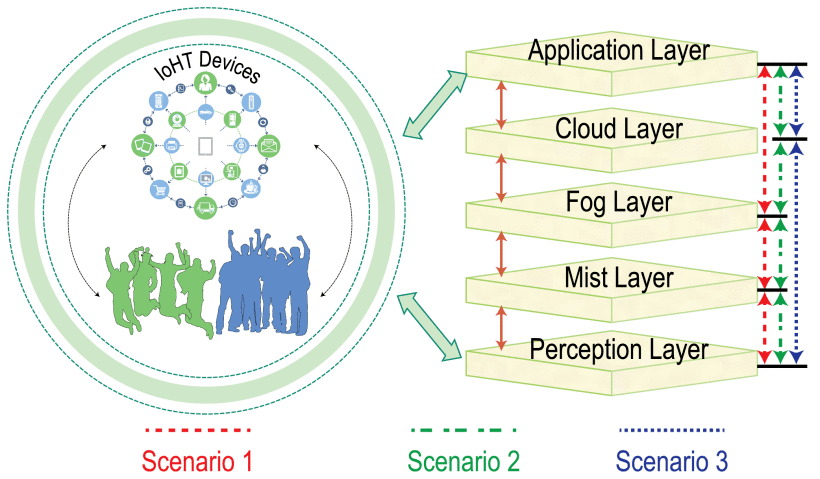
\includegraphics[width=\linewidth]{image/framework.png}
	\caption{IoHT Framework}
	\caption*{src:ASIF-UR-RAHMAN et al:\cite{3}}
\end{figure}

\subsection{The Components of 5-Layered Architecture}

\graphicspath{{C:/Users/LIKITHA/semitex/chapters}}
\begin{figure}[H]
	\centering
	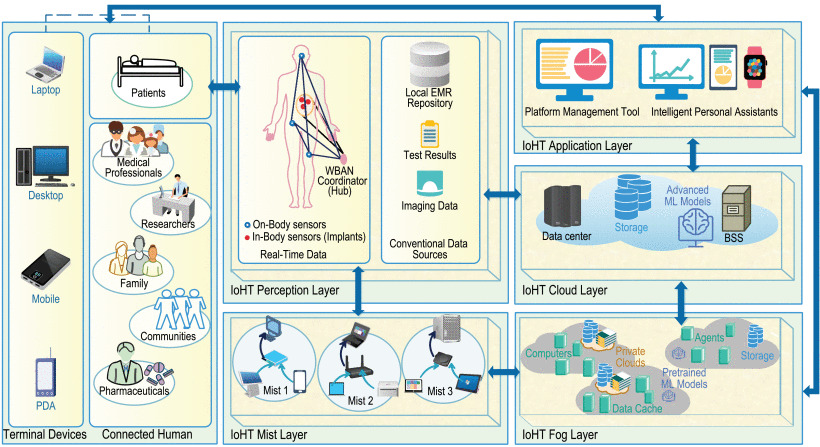
\includegraphics[width=\linewidth]{image/architecture.jpg}
	\caption{IoHT Framework Architecture}
		\caption*{src:ASIF-UR-RAHMAN et al:\cite{3}}
\end{figure}

Five Components of the framework are,\\
\begin{enumerate}
	\item Perception Layer
	\item Mist Layer
	\item Fog Layer
	\item Cloud Layer
	\item Application Layer\cite{3} 
\end{enumerate}


\subsection{Layers and their Goals}
\begin{figure}[H]
	\centering
	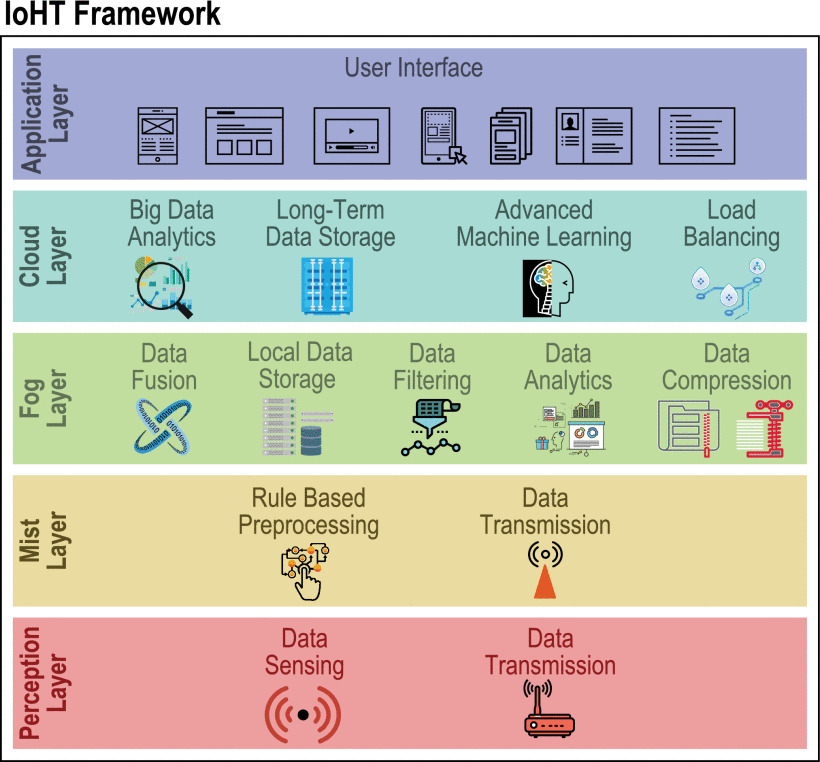
\includegraphics[width=\linewidth]{image/layered.jpg}
	\caption{Functionaities of 5-Layered IoHT Framework}
	\caption*{src:ASIF-UR-RAHMAN et al:\cite{3}}
\end{figure}

\begin{enumerate}
	\item Perception Layer:\\
	It is the lowest layer in IoHT Framework which identifies the devices that is connected to transmission and data gathering devices such as sensors,RFID tags,readers,medical imaging devices,etc which is inturn connected to the network and collects the data which is real-time as well as non-real time data.Otherthan realtime data there exists healthcare Big data such as (non)medical imaging data,electronic medical record(eMR),unstructured clinical notes etc which requires special handling because of their requirement of advanced data analytics.Based on the data type and processing requirements ,both kinds of healthcare data is transmitted to the next layer either to the Mist or Fog or Cloud\cite{3}.\\
	\item Mist Layer:\\
	In order to deal with critical time data processing,Mist was introduced in the model which stays inside the network fabric and operates at the edge of the network using sensors and actuator controllers and performs prepocessing based on rule based sensor data\cite{3}.Mist is responsible for optiml resource utilization of Things that have limited power,memory and communication bandwidth at the edge of IoT network.\\
	\item Fog Layer:\\
	In order to detect the anomalies(irregularities) and take immediate necessary actions by providing quick alarms at real time,Fog Layer was introduced.The fog layer is a decentralized architecture which ensures minimal latency and high responsiveness by bringing computing resources and application servers close together to the edge\cite{3}.This reduces latency and load on the cloud by local data storage,data compression,data filtering and intermediate data analytics that will improve QoS,System performance and save bandwidth.\\
	\item Cloud Layer:\\
	All healthcare data from fog layer and nonsensor sources such as eMR,eHR etc gets combined at Cloud layer for long-term storage, and big data and advanced analytics.The Cloud Layer is capable of connecting to Fog layer,Application layer and perception layer\cite{3}.It performs data analytics including machine learning,rule based processing,data mining and reasoning based algorithm to abstract meaningful data from healthcare data.\\
	\item Application Layer:\\
	It is the top most layer in IoHT framework that provides user interface between different stake holders and frameworks delivering many healthcare applications to the stakeholders and application developers by providing accesss according to the right and privilege from the cloud or fog layer directly\cite{3}.
\end{enumerate}

\subsection{Data processing \& Storage}
\subsubsection{Data-centric perspective}\\
\hfill\\ \\
In order to ensure smooth connectivity of heterogeneous data,a data centric transmission scheme has been made use of in the five-layered architecture.\\ \\
Depending on the availability of resource and data traffic,the processing load is assigned to either Mist or Fog or Cloud based on rule based Preprocessing, big data analytics,machine learning and etc in the 5-layered architecture.\\

The Below Flowchart describes the data transmission and processing that takes place at different layers of the IoHT Framework\cite{3}.\\

\begin{figure}[H]
	\centering
	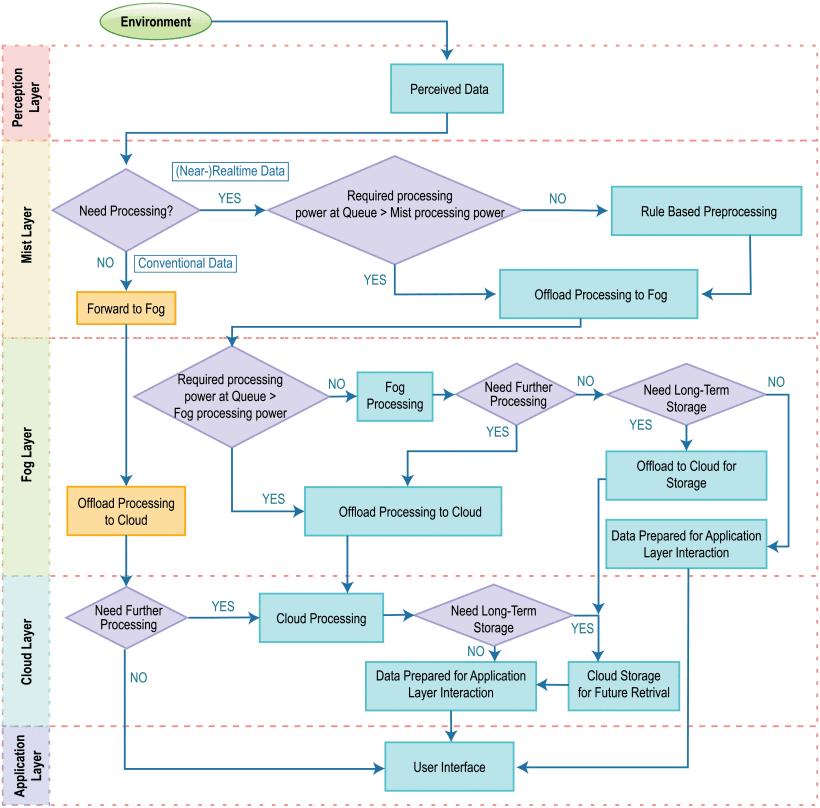
\includegraphics[width=\linewidth]{image/Datatransmission.png}
	\caption{Flowchart of data transmission and processing}
	\caption*{src:ASIF-UR-RAHMAN et al:\cite{3}}
\end{figure}

In order to achieve consistent communication among the heterogeneous data that is generated from perception layer in the proposed IoHT Framework,a data centric transmission scheme was maintained in order to deal with different types of data that was generated such as real time,near real time and offline mode(batch mode/Big data).To processing this data,it takes place in two different paths based on the traffic of data and availability of resource to attain better QoS,reduced latency and optimized power consumption\cite{3}.\\ \\

In case of real-time data,the data that is generated from the sensors that are located in the closest region and is first sent to Mist layer for processing and then forwarded to the next layer Fog which can deal with intermediate analytics and then the results are sent to application layer.

When the intermediate results sent by Fog layer is not sufficient,data is offloaded to the cloud layer which is capable of handling big data analytics,advanced machine learning,massive data generated by advanced medical instruments and etc and the data get stored in cloud for long term data storage that can be used further for reference.\\


\subsubsection{Networking}
The heterogeneous data generated from perception layer that can be real-time and non real time is sent to the nearest IoT hubs for processing.According to the processing rules and data traffic,it is then forwarded to either Mist or Fog or Cloud for preprocessing.In this process,the most critical aspect is to maintain QoS and that is achieved by deploying SDN(Software Defined Network)a programmable network structure that works on IoHT framework as centralized or decentralized for resource allocation,scheduling,routing and flow control through SDNC that uses network virtualization by decoupling control plane from data plane\cite{3}.\\

To attain better QoS,the network traffic is prioritized based on the transmission rate and delay and is classified as Delay-sensitive(DS),loss-sensitive(LS) and both delay as mixed(M)\cite{3}.\\

A sample data of IoHT healthcare traffic classification is as shown below.\\

\begin{figure}[H]
	\centering
	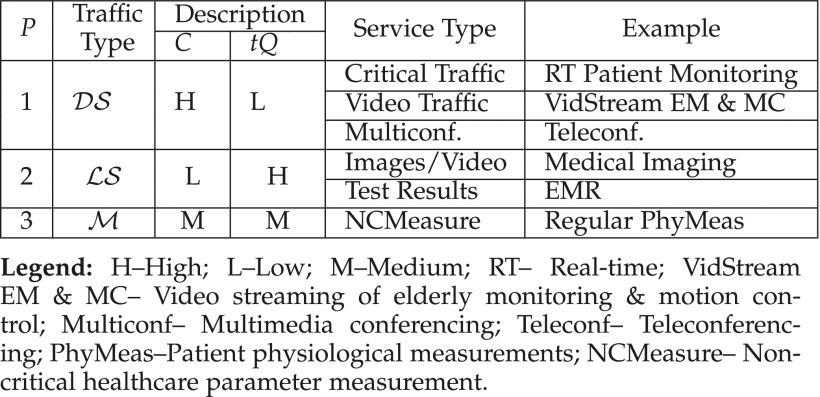
\includegraphics[width=\linewidth]{image/Table.png}
	\caption{Flowchart of data transmission and processing}
	\caption*{src:ASIF-UR-RAHMAN et al:\cite{3}}
\end{figure}
\newpage
\subsection{Data Analytics \& Machine Learning}
With the evolution of IoHT in recent years,traditional databases cannot handle the huge data and there is a huge hype for Machine Learning methodologies and Data Analytics to be used to deal with the voluminous data generated by the sensors and IoHT devices in order to provide useful and innovative process to the industries for cost cutting and improved approaches helping their business models achieve a better experience by enabling a parallel execution and distribution of data on multiple servers.\\ \\
The voluminous data generated by the IoHT devices require special methods and approach for handling and processing the structured and unstructured data.Machine learning plays an important role in IoHT Framework which is capable of handling the decisions based on certain Machine learning alogorithms where it can provide services with faster analysis and expert intervention for better treatment recommendations for the monitor of diseased person.By using machine learning methods in devices,it firstly works towards the goal irresppective of the factors that can impede and later decides the important input variables required to achieve the goal and predict the future events ensuring prevention before hand.\cite{syed2019data}\\ \\
Although data analytics could be made use of for measuring success overtime by providing smarter decision and generates report based on the data that was collected,it is not appropriate for IoT as data analytics is often static having limited-use in addressing fast-changing and unstructured data.\cite{calum}But Machine learning addresses the fast changing and unstructured data by focusing on the outcome fisrt and later decides automatically which variables is required and their interactions accordingly based on certain algorithm implementation.\\ \\
Machine Learning is not just used for machines and devices where maintainence is automated but humans too,for calling an emergency support automatically when in need.\\ \\

Example :\\ Diastolic/sistolic pressure alert event\\
High Blood pressure is one of the crucial factors that leads to stroke.Hence continous monitoring of blood pressure anytime anywhere is very essential in order to prevent and predict stroke before hand.\cite{ma2014blood} According to one of the research,a calibration method using machine learning algorithms was made use of in order to detect the variation of pulse transit time by detecting automatically the compensatory movements based on sensors and camera based devices around the patient.By continuously monitoring the patient,with an average of 0.5$\pm$3.9mmHg for systolic and diastolic blood pressure\cite{ma2014blood},an aleart event will be sent when it reaches the above average blood pressure to the caretaker through the monitoring tool that can ensure high prevention and help well in hand.

\newpage
\section{Case Study \& Evaluation based on Taylor James paper}
\subsection{Weakness of the paper/Missing Elements}
According to the research paper by Taylor,IoT is an emerging technology that supports global infrastructure for exchange of information between ubiquitous computing devices without any interaction of humans. This paper describes the importance of practical and intelligence of Iot applications majorly in healthcare sector using a 5-Layered Architecture that represents its functionalities in an effective way.However there are few other factors that must be take care of such that IoHT devices can work efficiently\cite{5}.\\ \\
Few factors that require considerations are,
\begin{enumerate}
	\item Implementing Classical Middleware approach - Publish \& Subscribe method\\
	\item Introduction to Docker/Kubernetes\\
	\item Ensuring Privacy \& Security\\
\end{enumerate}
\subsubsection{Classical Middleware Approach-Publish\&Subscribe}
\hfill\\
\hfill\\
\emph{How can middleware approach of Publish \& Subscribe method help IoT Platform to meet their requirements?}\\ \\
IoHT comprises of various ubiquitous devices and technologies that offers real time data transmission of the surrounding and provide triggers based on the changes in the physical world.This methods lead to the approach of smart Healthcare,smart city,smart application and etc where billions of devices are connected over the internet for seemless interoperability.\\ \\
The classical sensor based devices deployed in IoT provide real time data but few devices have constraint where they can read the sensor data only once,which should be later distributed to several applications/services.To handle this challenge,a scalable cloud based messaging layer\cite{happ2017meeting},Publish and Subscribe model is used,that can match the data stream to the interested applications and distribute data accordingly.\\ \\
Pub/sub system mechanism ensures high performance processing and interoperability to allow devices to publish their presence(send data)to the node called as broker/router,which is responsible for traffic handling and distribution of data,and on the other side devices can subscribe to the broker for accessing the information based on their requirement.\\ \\
Pub/Sub is an asynchronous messaging service that decouples services that produce events from services that process events.It ensures message storage and real-time message delivery with high availability and consistent performance at high scale\cite{6}.\\ \\
Integrating publish/subscribe method in IoT platform is considered as the best approach for the interoperability and 
distributing various kinds of data over the network on different layers that acquires data from various other devices such as entities,devices,wireless sensors and etc.\\

\begin{figure}[H]
	\centering
	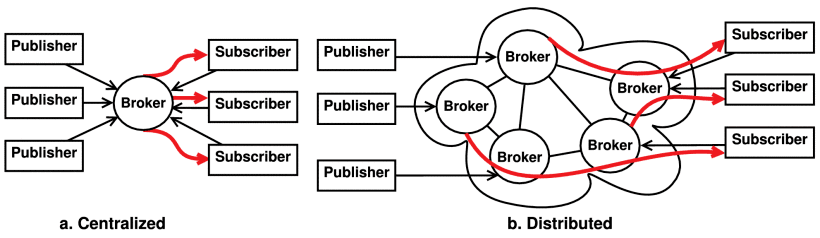
\includegraphics[width=\linewidth]{image/pub-sub.png}
	\caption{Publish-Subscribe System}
	\caption*{src:ElHassan et al\cite{4}}
\end{figure}

The usage of sensors and wireless technology for communication between the devices has lead to increased importance of wirless sensored networks in IoT.\\
Centralized pub/sub is more suitable for small network enterprise where as in case of large network consisting of many devices and heterogeneous data that uses topic-based filtering, Distributed pub/sub is very appropriate\cite{4}.\\ \\
Example:\\
PubSub thermostat: Controlling the fan based on the temperature change in IoT system,where the devices in this system publish temperature data on their pubsub registry feeds and individual device IDs. A server python application, which can run from any machine, consumes the data from Cloud based on Pub/Sub topic and events. The server then decides whether to turn on or off the individual devices fans via a Cloud IoT Core configuration update\cite{matthew}.
\subsubsection{Docker/Kubernetes}
\hfill\\
\hfill\\
\emph{Why is docker/kubernetes required in IoT Framework?}\\ \\ 
In recent years, cloud computing is an emerging field that deals with wide range of highly connected smart devices such as medical trackers,sensors,home appliances,and etc providing high computing power at low management effort.\\
As the developers deal with large number of devices,using containers can help them is many ways.\\ \\
Containers are lightweight when compared to virtual machines that uses lightweight kernel namescapes and runs on Build,Ship and Run Paradigm and virtualize the operating system and not the hardware which can enable applications run in isolation without affecting other applications making easy to move,modify and deploy with high security and scalability.\\ \\
The main idea of containers is to collect all the tools and libraries necessary to run a specific piece of software, and then isolating that software from the rest of the system. Because containers are not full-on virtual machines, they’re efficient, and Docker which is lightweight,standalone, is a leader in making containers easy to work with and share with others by ensuring better security and easy development\cite{8}.\\ \\

\begin{figure}[H]
	\centering
	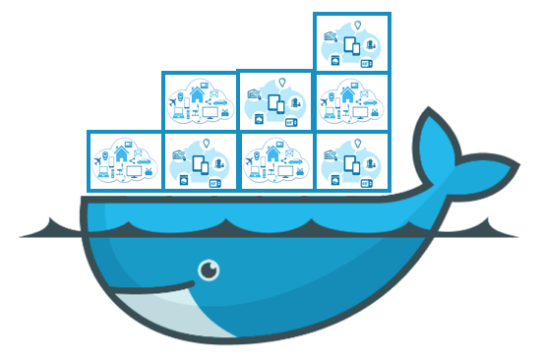
\includegraphics[width=10cm]{image/iot_containers.png}
	\caption{Docker Containers and IoT applications}
	\caption*{src:\cite{docker}}
\end{figure}

Docker,"the worlds leading software container platform and a tool that helps to solve common problems like installing,removing,upgrading,
distributing,trusting and managing software and provides a modern solution to tackle common software problems"\cite{7}.\\ \\
It is easy to maintained and deployed upon the virtulization machines.In IoT Framework,Applications that run different services on many devices make it reasonable to utilize a technology providing easy deployment and high portability within a distributed system environment\cite{7}.\\ \\
By using docker,the main challenges in IoT devices can be solved by enabling minimal hardware resources,highly scalable,distribution across the network,
limited network access and heterogeneous device environments.\\ \\
\begin{figure}[H]
	\centering
	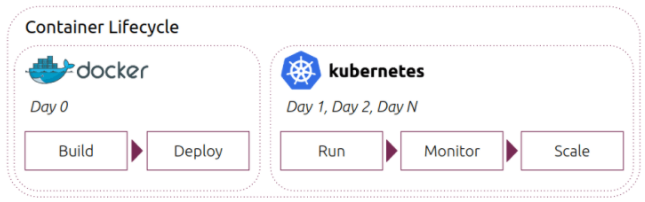
\includegraphics[width=\linewidth]{image/dockub.png}
	\caption{Docker and Kubernetes}
	\caption*{src:\cite{kub}}
\end{figure}
To automate these functionalities on a large scale,Kubernetes,an open source platform is what is required which gives system admin more control on the containers for deploying,scaling,managing and automates the processes in containerized application.Kubernetes benefits IoT as developers need not worry about the hardware or opeating system specifications and the property of self-healing makes the system more robust and reliable.With this ability,healthcare organizations in IoT platform implement both docker and kubernetes technology to reduce cost and time,provide high security,self-healing,quick deployment of application and highly scalable.\\ \\


\subsubsection{Privacy \& Security}
\hfill\\
\hfill\\
\emph{Why privacy and security is important in IoT?}\\ \\
Privacy and security is one of the key challenges faced by IoT in order to ensure secure and encrypted communication among billions of devices collecting data through wireless network.Most of the security issues faced during communication are Malicious code injection,sniffing attack,Denial of service,proxy attack and etc.There are few other factors such as proxy attack and man-in-the-middle attack that occurs irrespective of the connectivity being encrypted or not\cite{sec}.Hence it is necessary to ensure a secure and reliable communication protocols at all stack layers.\\ \\

\begin{figure}[H]
	\centering
	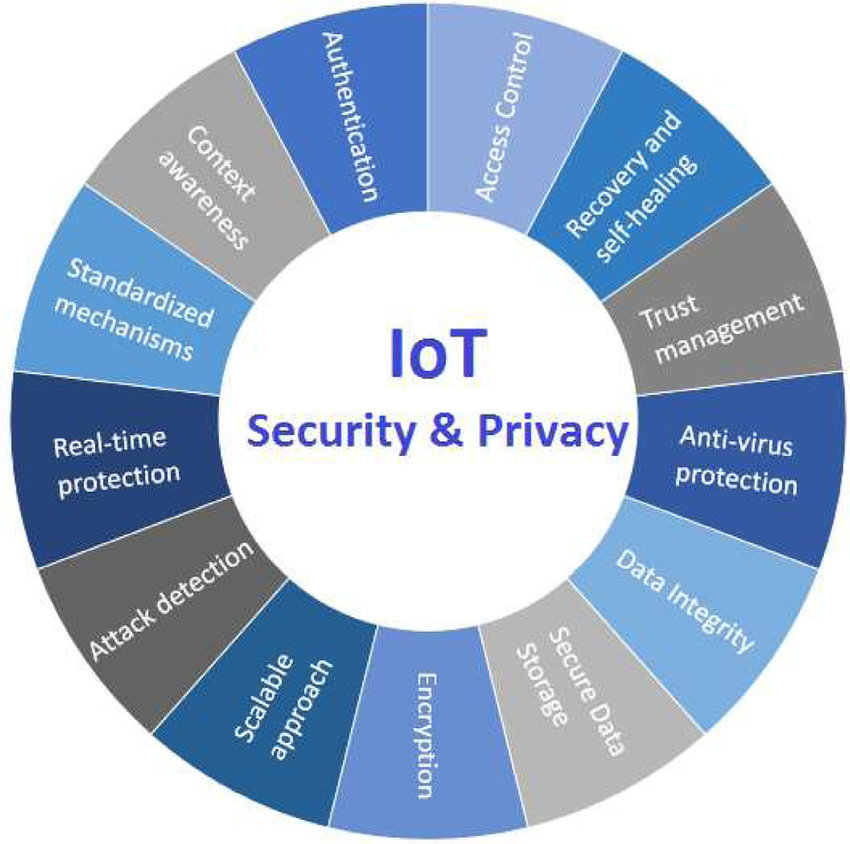
\includegraphics[width=8cm]{image/security.png}
	\caption{IoT security and privacy concerns}
	\caption*{src:\cite{sec}}
\end{figure}

The new Fog computing framework allows storing and processing the data at edge/cloud-to-endpoint continuum by overcoming the limitation of IoT devices.In general distributed systems are more vulnerable to attacks when compared to centralized systems.\\
Cloud usually operates in heavily protected facilities and managed by cloud operators where as Fog needs to function in more vulnerable environments by meeting customers requirements.As fog has resources smaller when compared to cloud it may not protect itself because of limilited resources.\\
Hence there are many privacy and security issues in Fog architecture that has to be addressed such as authentication,secure communication,confidentiality and authorization.\\
Inspite of cloud-platform providing advanced cryptosystem to enhance security,it cannot be implemented on resource-constraint devices in Fog as many devices are located in various locations and the chances of malicious activities are high\cite{9}.\\
 %https://www.hindawi.com/journals/wcmc/2018/9373961/
In order to deal with such problems,WebRTC(Web Real time communication) an open-source web-based application technology,is made use of which has the ability to deal with security issues in real-time communication by enabling and encouraging important security concepts at stack level.OpenTrust Protocol(OTrP) is used by applications to install,update,delete and manage security configurations.IPSec(Internet Protocol Security) is used in network layer which provides a end to end secure and transparent connection-oriented channel is used which is easier to run than TLS(Transport Layer security).Few applications rely on SSl(Secure socket layer) and DTLS(Datagram Transport Layer security) for secure data transmission.To deal with the Man-in-middle attack, media paths should be regularly monitored and should be coupled with encrypted signals for no spectical threat\cite{sec}.\\ \\
As the system grows large with enoromous data,it is always benificial to adapt lightweight protocols and encryption algorithms for better security in IoT environments and each object should check other's privacy policy for compatability before sharing data,as each system has its own privacy policies.Security and privacy is no longer an option but a must requirement in all fields.

\newpage
\section{Conclusion}
The Rapid development in the field of internet and tehnology, IoT is changing our life by making things smarter and easier than ever before.According to Taylor\cite{3},the proposed five-layered IoHT Framework consisting of perception,mist,fog,cloud and application layer provides an efficient,sustainable and evolved features by widening the boundries of internet for the interoperability between devices for anything,anytime and anywhere with advanced computing speed and scalability for usability in IoHT smart applications by enabling seperate routing paths to handle the real-time as well as conventional data generated by IoHT devices.This can help modern healthcare industries grow widely by providing services to the users through eHealthcare services inspite of reduced workforce.This also emphazises the importance of adapting modern technologies such as machine learning and data analytics to handle the increased complexity in computational analysis and ensure high QoS with low packet drop from the data generated by large heterogeneous medical devices and organizations. Also focuses on implementing few other factors such as privacy \& security,usage on virtualization container technologies such as Docker \& Kubernetes and making use of few middleware technologies such as Publish/subscribe system to the already existing famework that can help IoHT Framework work seemlessly with effective performance and scalable distribution of data for the IoHT based healthcare systems.
%
%===============================================================================
% LATEX-Dokument: Literaturverzeichnis
%===============================================================================
%
\newpage
\phantomsection
% Einstellungen f\"{u}r Literaturverzeichnis
\addcontentsline{toc}{section}{\bibname}

\bibliographystyle{IEEEtran}
% argument is your BibTeX string definitions and bibliography database(s)
\bibliography{literature/bib}
% Nutzung von Bibtex:
% hier den bib-file einbinden
%
% GATHER{bibfile.bib}
% \footnotesize
% \bibliography{bibfile}
% ansonsten: bbl als tex Datei einbinden
 %\input{KTR-Seminar-Literatur.tex}
%===============================================================================
% LATEX-Dokument: Literaturverzeichnis
%===============================================================================
%
\end{document}
